\subsection{Disparity Testing}
After the camera interface was verified as functional, a large portion of time was spent implementing a disparity algorithm that allowed for the extraction of 3D depth information from stereo image data. This algorithm was first implemented in \textsc{Matlab}, and was then re-designed to operate within programmable logic. 

\subsubsection{Image Rectification}
In order to perform the most accurate block matching possible on camera image data, it would have been ideal to rectify the images as outlined in Section \ref{rectsec}. However, since the image data used in the disparity calculation contained a central 384x288 image taken from the middle of each 752x480 input image, a large portion of the input image was cropped out. Since many of the lens artifacts corrected using a rectification process are contained on the external edges of the input imagery, no additional camera calibration was performed in the disparity or camera controller implementations \cite{collins}. 
\par
After extensive testing with the stereo camera breakout board and disparity module detailed in the following sections, it was also found that camera imagery captured from the stereo camera interface contained consistent horizontal epipolar lines between both images. These lines were accurate enough for the custom disparity algorithm to process without additional calibration, saving a large amount of calibration time in the image processing pipeline. With the issue of camera calibration and image rectification addressed, it was then possible to begin implementing a test disparity algorithm in \textsc{Matlab}.

\subsubsection{\textsc{Matlab} Implementation}
The Sum of Absolute Differences algorithm discussed in Section \ref{SADexample} was first implemented using \textsc{Matlab}, and can be found in Appendix item \ref{disparityTestMatlab} \cite{mccormick}. This implementation operated on the "cones" standard test image set, and produced a resultant disparity image from the given input image pair. In the case of this specific example, the algorithm performed a 7x7 Sum of Absolute Differences block matching process on 50-pixel search ranges across horizontal epipolar lines between the two images. Note that the block size and search range were also implemented so that they could be customized by the user to test the algorithm's functionality. 
\par
Overall, the \textsc{Matlab} disparity test implementation was broken down into the following steps:
\par
\singlespacing
\begin{enumerate}
\item
Load in image data (also convert to grayscale if using the "cones" image set)
\item
Determine the size of the template image and create a resultant matrix to store output disparity values in
\item
For each full row of pixels across an image, perform the following steps:
\begin{enumerate}
\item
Set minimum and maximum row bounds for the current block of pixels being used for SAD 
\item
For each column in the given row, perform the following steps:
\begin{enumerate}
\item
Set minimum and maximum column bounds for the current block of pixels being used for SAD
\item
Determine the number of blocks that will be used in the current search. Note that this number will be the Disparity Range until the blocks being searched are closer in pixels to the right edge of the image than the Disparity Range
\item
Create a memory block for holding the SAD value for each block comparison based on the number of blocks from (ii), and create a template block from the right image at the current column/row
\item
For the number of blocks calculated in (ii)
\begin{enumerate}
\item
Compute the Sum of Absolute Differences for each left image block along the current pixel row with respect to the right image template block, and store the calculated value in the memory block created during (iii)
\end{enumerate}
\item
Find the smallest value in the memory block containing SAD values. Use the index of this block to determine the pixel offset from the template block location. This value is the disparity for the particular point
\item
Store the calculated disparity value in the resultant image matrix. Go back to (b) if there are more columns (pixels) remaining in the current row, otherwise go to (3)
\end{enumerate}
\end{enumerate}
\item
When the entire image has been iterated through, display the resultant disparity matrix, and scale pixel coloration based on the minimum and maximum disparity values for better contrast.
\end{enumerate}
\doublespacing
\par
An example of a resultant disparity image from this test implementation is shown in Figure \ref{dispMatlabOutput} below.
\begin{figure}[H]
	\centerline{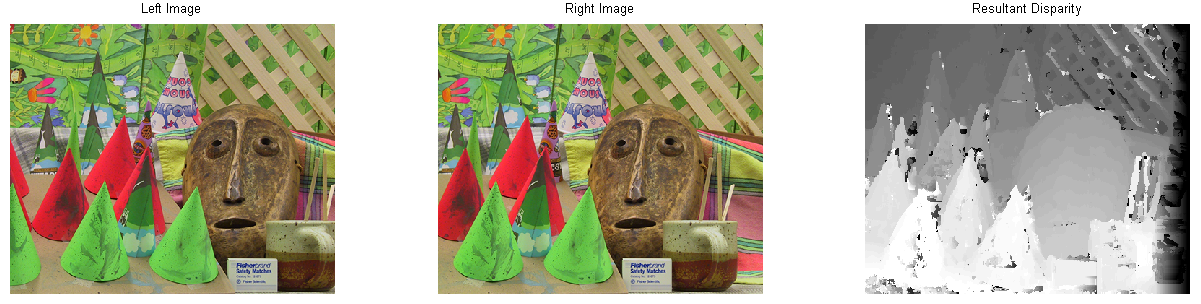
\includegraphics[width=1.2\textwidth]{disparity.png}}
	\caption{Disparity Implementation Output}
	\label{dispMatlabOutput}
\end{figure}

\subsubsection{Verilog Test Bench}
The original Verilog disparity test implementation used closely followed the \textsc{Matlab} disparity algorithm discussed in the previous section. This algorithm was implemented using a finite state machine with five states, as shown in Figure \ref{disparityTestImp} below. To maintain simplicity for initial testing, the test algorithm originally operated on the 20x7 pixel test images shown in Figure \ref{disparityTestImg}. The search range and block size for this module were set to 15 pixels and 5x5 pixels, respectively. By default, the disparity module remained in an idle state until an external enable signal was toggled high using a button input. This caused the finite state machine to advance to its READ state, and image data for the left and right camera images was then read in from the stereo camera breakout board. After image data was received, the state machine would then advance to a cyclical set of states used for iterating through each image and calculating disparity. 
\par
\begin{figure}[H]
	\centerline{
\includegraphics[width=0.75\textwidth]{disp_tb/testImages.png}}
	\caption{Disparity Test Images}
	\label{disparityTestImg}
\end{figure}
The disparity module would begin by isolating the template and search blocks from the right and left image data in the finite state machine's separation state. Next, the state machine would advance to its SAD state, and calculated the Sum of Absolute Differences between the template and search block. The SAD value was then placed in a vector that matched the length of the search range, with a vector index that corresponded to the current pixel location being searched. If the vector was not completely filled, indicating that there were more search blocks to compare to the template, the state machine would revert back to the separate state, isolating a new search block from the right camera image. When the SAD vector was full, the state machine would then advance to its finalization state. 
\par
\begin{figure}[H]
	\centerline{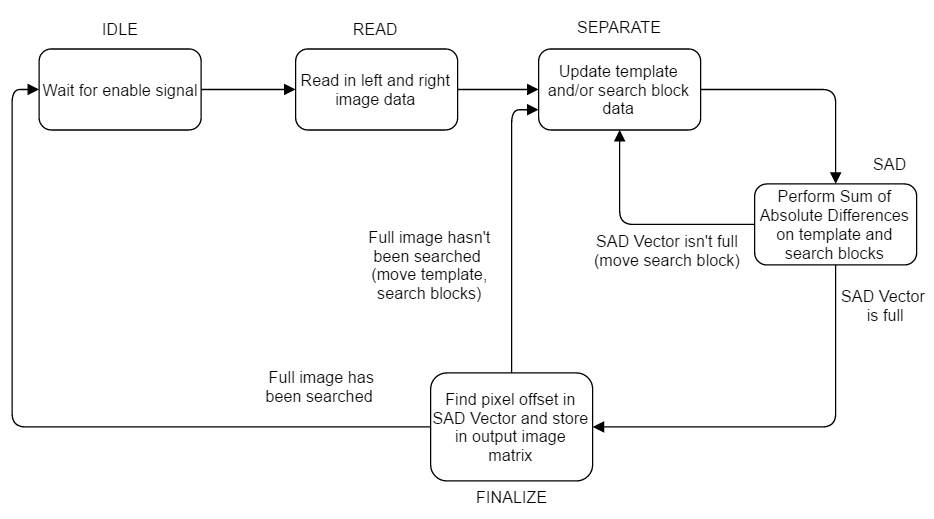
\includegraphics[width=1.0\textwidth]{looping_disparity.png}}
	\caption{Disparity Test Implementation}
	\label{disparityTestImp}
\end{figure}
\par
The finalization state was used to search through the SAD vector for the lowest value. The index of this value within the SAD vector was equivalent to  a disparity value for the given template block location. This value was  converted to a distance measurement using Equation \ref{disp2dist}, and was stored in the output image location. If the output image was not fully populated with distance values, the state machine reverted back to the separate state. Otherwise, the state machine advanced to its idle state, indicating that the resulting disparity image was ready for output. 
\par
This module was initially tested using a Verilog Test Bench, and was then tested using camera image data and a VGA display controller module, allowing for real-time verification of the algorithm's effectiveness. After testing the initial disparity algorithm, several modifications were made to increase the overall speed and efficiency of the disparity module. 
\subsubsection{Test Bench Results}
The READ state of the disparity state machine was first analyzed using the Verilog Test Bench, and the these test results are shown in Figure \ref{disparityImgRead} below. The state machine is shown transitioning from IDLE (0) to READ (1) in the beginning of the timing diagram, as indicated by \texttt{state\_LED}. After transitioning to its READ state, the disparity module read in each image horizontally from left to right, as dictated by \texttt{buffer\_href} and \texttt{buffer\_vref}. The left camera image was read first, and output \texttt{image\_sel} was then toggled to signal a second read sequence from the right camera image buffer. During each rising clock cycle, input \texttt{image\_data} was stored in an internal BRAM module for the associated camera's image data, with the write address based on the current value of \texttt{buffer\_href} and \texttt{buffer\_vref}. 

\par
\begin{figure}[H]
	\centerline{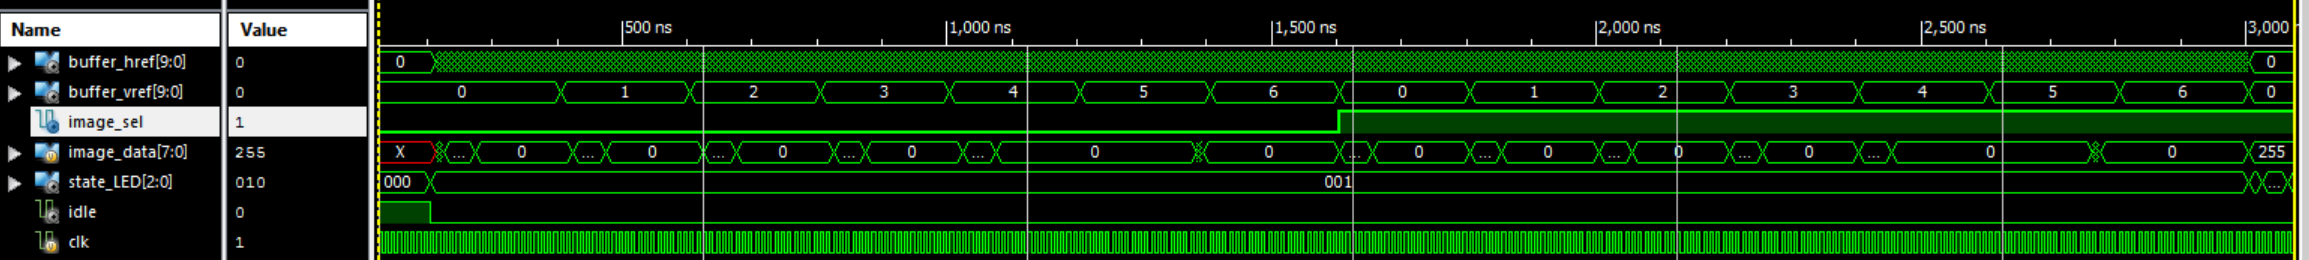
\includegraphics[width=1.25\textwidth]{disp_tb/read_bothimages.png}}
	\caption{Image Read Sequence}
	\label{disparityImgRead}
\end{figure}
\par
After the state machine finished reading both images into local memory, it then iterated through the SEPARATE (2) and SAD (3) states until an entire search range of search blocks had been compared to the given template block. After the search range had been traversed, the state machine advanced to its FINALIZE (4) state to find the disparity value for the given search and place the value in the output buffer. Figure \ref{disparityVector} shows an example of this process, where a template block set by pixel row bounds \texttt{minr} and \texttt{maxr} and pixel column bounds \texttt{t\_minc} and \texttt{t\_maxc} was compared to 15 individual search blocks set by row bounds \texttt{minr} and \texttt{maxr} and column bounds \texttt{b\_minc} and \texttt{b\_maxc}.
\par
\begin{figure}[H]
	\centerline{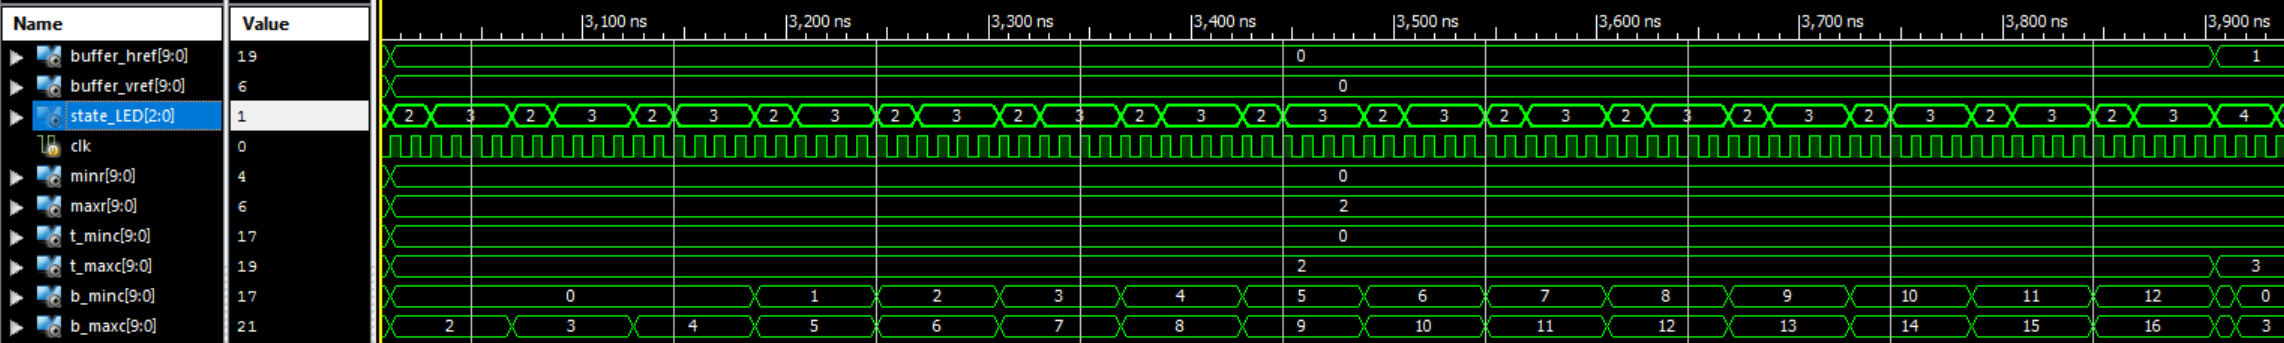
\includegraphics[width=1.25\textwidth]{disp_tb/disparity_vector.png}}
	\caption{Disparity Search Vector}
	\label{disparityVector}
\end{figure}
\par
Note that in the case of the disparity search shown in Figure \ref{disparityVector} above, a disparity value was calculated for the pixel location (0,0), or the top left corner of the image, as defined by \texttt{buffer\_href} and \texttt{buffer\_vref}.
\par
After each disparity search was completed, the state machine then advanced from the FINALIZE state to the SEPARATE state to isolate a new template block and search block. Internal counters for horizontal and vertical pixel location of the disparity search were also updated at this point, triggering an update of the template and search block parameters, as well as the number of blocks analyzed in the current disparity search. This number decreased as the template block approached to the right side of the image, since the search range eventually exceeded the distance from the template block to the far width (right edge) of the image. An example of multiple disparity searches across one horizontal line of pixels in the top row of the 20x7 test image from Figure \ref{disparityTestImg} is shown below in Figure \ref{disparityHorizSearch}. In the case of this example, \texttt{numBlocks} represented the number of blocks included in the current disparity search. Since the width of the test image was 20px and the search range was set to 15px, \texttt{numBlocks} began to decrease after the 4th disparity search was performed, as shown below.
\par
\begin{figure}[H]
	\centerline{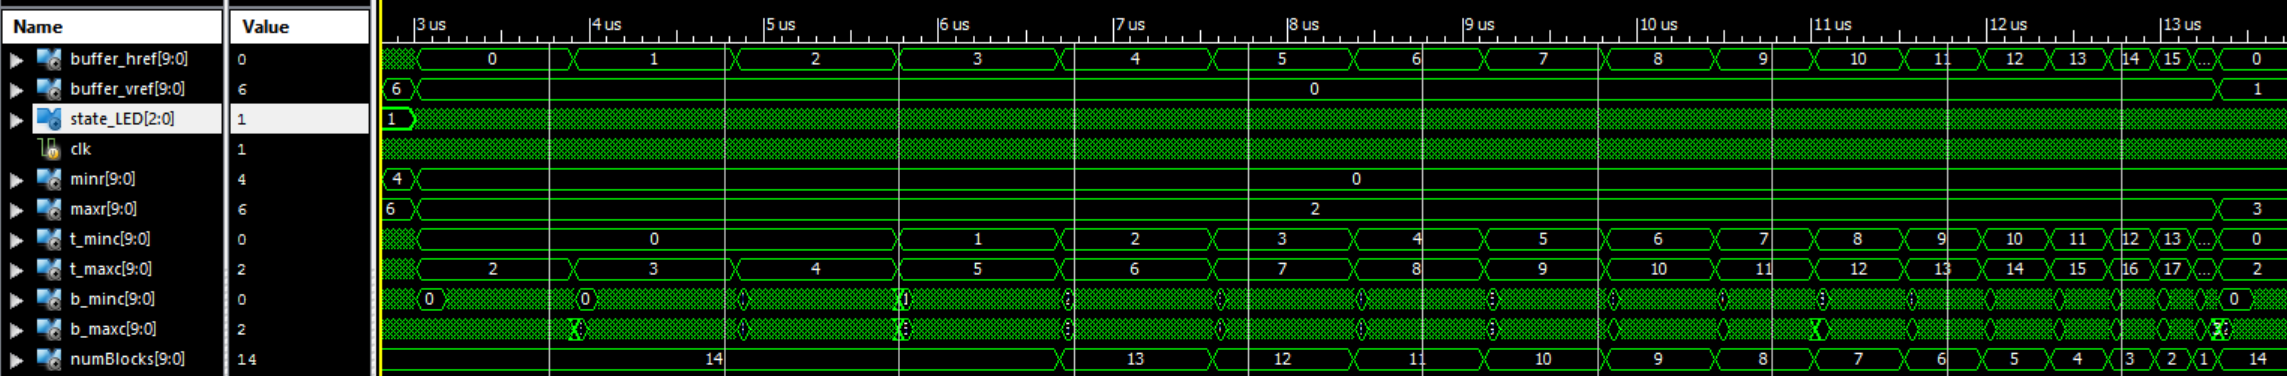
\includegraphics[width=1.25\textwidth]{disp_tb/disparity_fullPixelRow.png}}
	\caption{Horizontal Pixel Row Search}
	\label{disparityHorizSearch}
\end{figure}
\par
After an entire horizontal row of pixels was analyzed by the disparity algorithm, the vertical location of the template block was increased, and the overall process was repeated continuously until the entire image was analyzed. An example of a disparity search through the entire 20x7 image is shown below in Figure \ref{disparityFullSearch}.
\par
\begin{figure}[H]
	\centerline{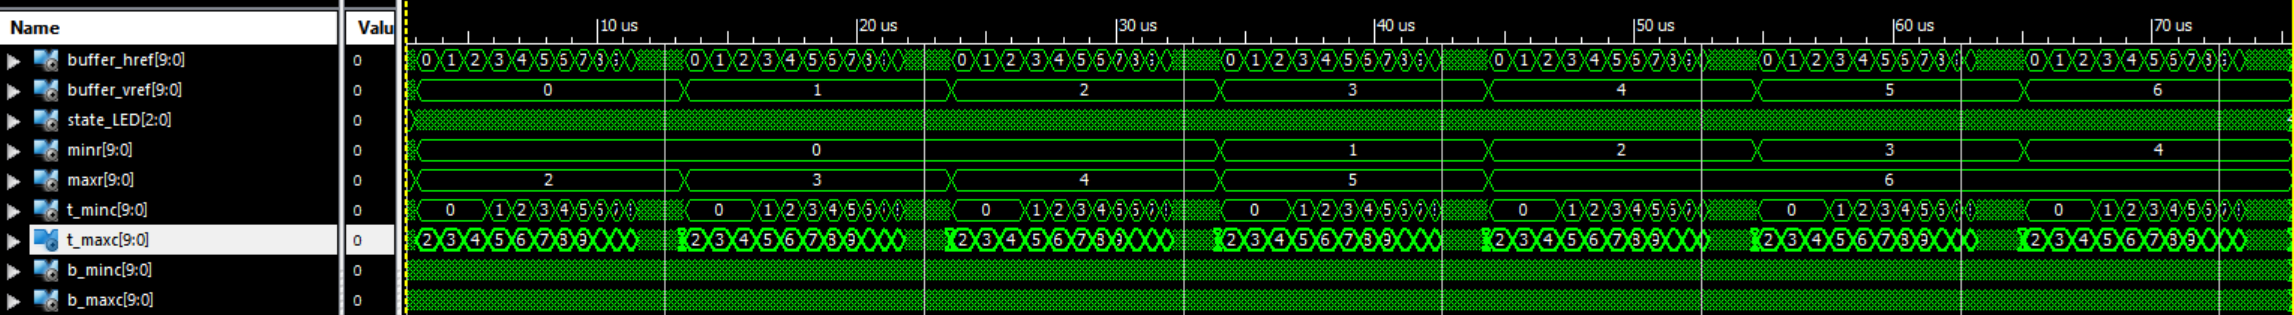
\includegraphics[width=1.25\textwidth]{disp_tb/full_disparity.png}}
	\caption{Full Image Search}
	\label{disparityFullSearch}
\end{figure}
\par
The output disparity image from the test analyzed above is shown in Figure \ref{disparityTestResults}. Note that the artifacts in the resultant image were due to the fact that a 5px$*$5px template and search block set was used on a 20px$*$7px image. The relatively large block size used in comparison to the size of the image made it impossible for any block comparison to avoid the block contained in the upper left corner of the search image. In addition, the direction of artifacts around the block in the lower right corner of each image were a function of the search direction, since the search blocks descended downwards and to the left.
\par
\begin{figure}[H]
	\centerline{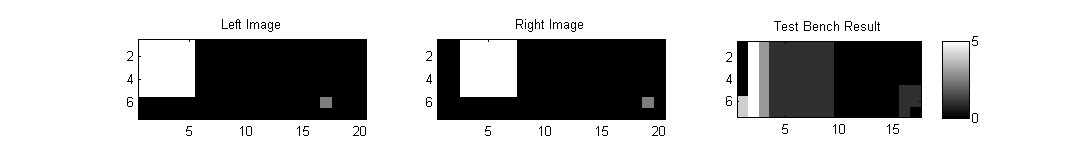
\includegraphics[width=1.0\textwidth]{disp_tb/result_gray.png}}
	\caption{Disparity Test Results}
	\label{disparityTestResults}
\end{figure}
\par
After the disparity module was deemed working on the 20x7 test image, further testing on image data was performed. First, a \textsc{Matlab} script for converting image data to a format recognizable by the Verilog Test Bench's \texttt{\$readmemb} command was created. Using these converted images, the Verilog disparity implementation's results were compared to those of the \textsc{Matlab} implementation. Note that due to limitations in computer memory, the disparity search range and block sizes capable of being processed by the Verilog Test Bench were limited to 15 pixels and 5x5 pixels, respectively. 
\par
Figure \ref{disparityVerilogvsMatlab} below contains a comparison between the test bench and \textsc{Matlab} results from disparity search on the "cones" test image set. Note that the outputs from the \textsc{Matlab} and Verilog disparity search algorithms were noticeably close in comparison, as well as in pixel intensity. Losses in the the output of the Verilog disparity algorithm were likely due to the fact that all operations were performed using integers rather than floating point values.
\par
\begin{figure}[H] 
         \begin{subfigure}[h]{0.5\textwidth}
              \centerline{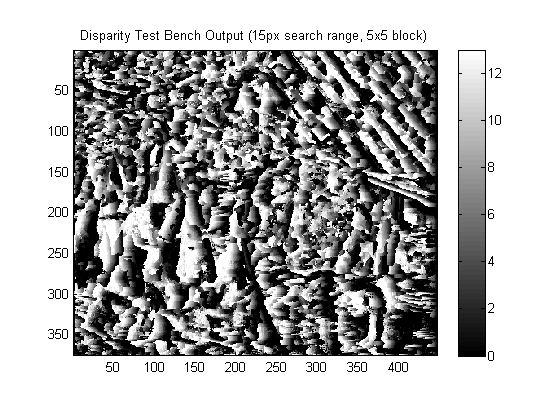
\includegraphics[width=1.1\textwidth]{disp_tb/tb_cones.png}}
             \caption{Test Bench Result}
         \end{subfigure}
         \begin{subfigure}[h]{0.5\textwidth}
             \centerline{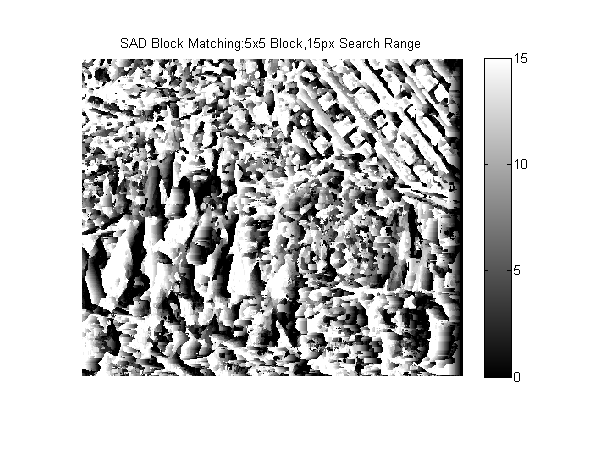
\includegraphics[width=1.1\textwidth]{disp_tb/MATLAB_conesDSP.png}}
             \caption{\textsc{Matlab} Result}
         \end{subfigure}
\caption{\textsc{Matlab} vs. Verilog Test Bench Results}
\label{disparityVerilogvsMatlab}
\end{figure}
\par
After the disparity implementation was fully tested in programmable logic using a Verilog Test Bench, a modified version of the implementation was created for final use. 

\subsubsection{Final Disparity Implementation}
Several structural changes were made to the original disparity implementation in order to create a finalized module for use in the overall system. In order to increase the speed of the disparity algorithm's output, several portions of the Verilog module used in the previous section were modified for increased parallelization and decreased overall latency associated with vectorized summation calculations. Most of this parallelization consisted of modifying 2D memory arrays used for storing the template and search blocks, and breaking said arrays into individual vectors. For example, instead of using a 7x7 memory array for storing one "block" of pixels, the block was broken into seven separate 1x7 vectors that were then operated on individually. This parallelization decreased the overall latency of the system by reducing time spent waiting to read from individual addresses within memory arrays. An overall block diagram of the parallelized disparity implementation is shown in Figure \ref{disparityFinalImp} below. 
\par
\begin{figure}[H]
	\centerline{\includegraphics[width=1.2\textwidth]{Disparity_Algorithm.png}}
	\caption{Disparity Final Implementation}
	\label{disparityFinalImp}
\end{figure}
\par
The overall state machine used to create the final disparity implementation still followed the same next-state logic as that of the original implementation shown in Figure \ref{disparityTestImp}. Advances in speed of the overall algorithm were therefore mostly associated with parallel calculations during the computation of the Sum of Absolute Differences. As discussed in Section \ref{dataman}, the left and right search images passed to the disparity algorithm were also windowed to $0.6\times{}VGA$ resolution, further reducing computation time. 
\par
The disparity hardware implementation was debugged by passing the current state of the disparity state machine to the ZedBoard's LEDs. Another important debugging step included a VGA output mode that showed the current camera images being used by the disparity algorithm. An example of this mode's output is shown in Figure \ref{camOutMode}. This example image shows a lab bench to the left, with a chair and doorframe on the right. Note that the image coloration was a result of mapping a monochrome image to arbitrary VGA colors to account for a lack of grayscale color space.
\par
\begin{figure}[H]
	\centerline{
	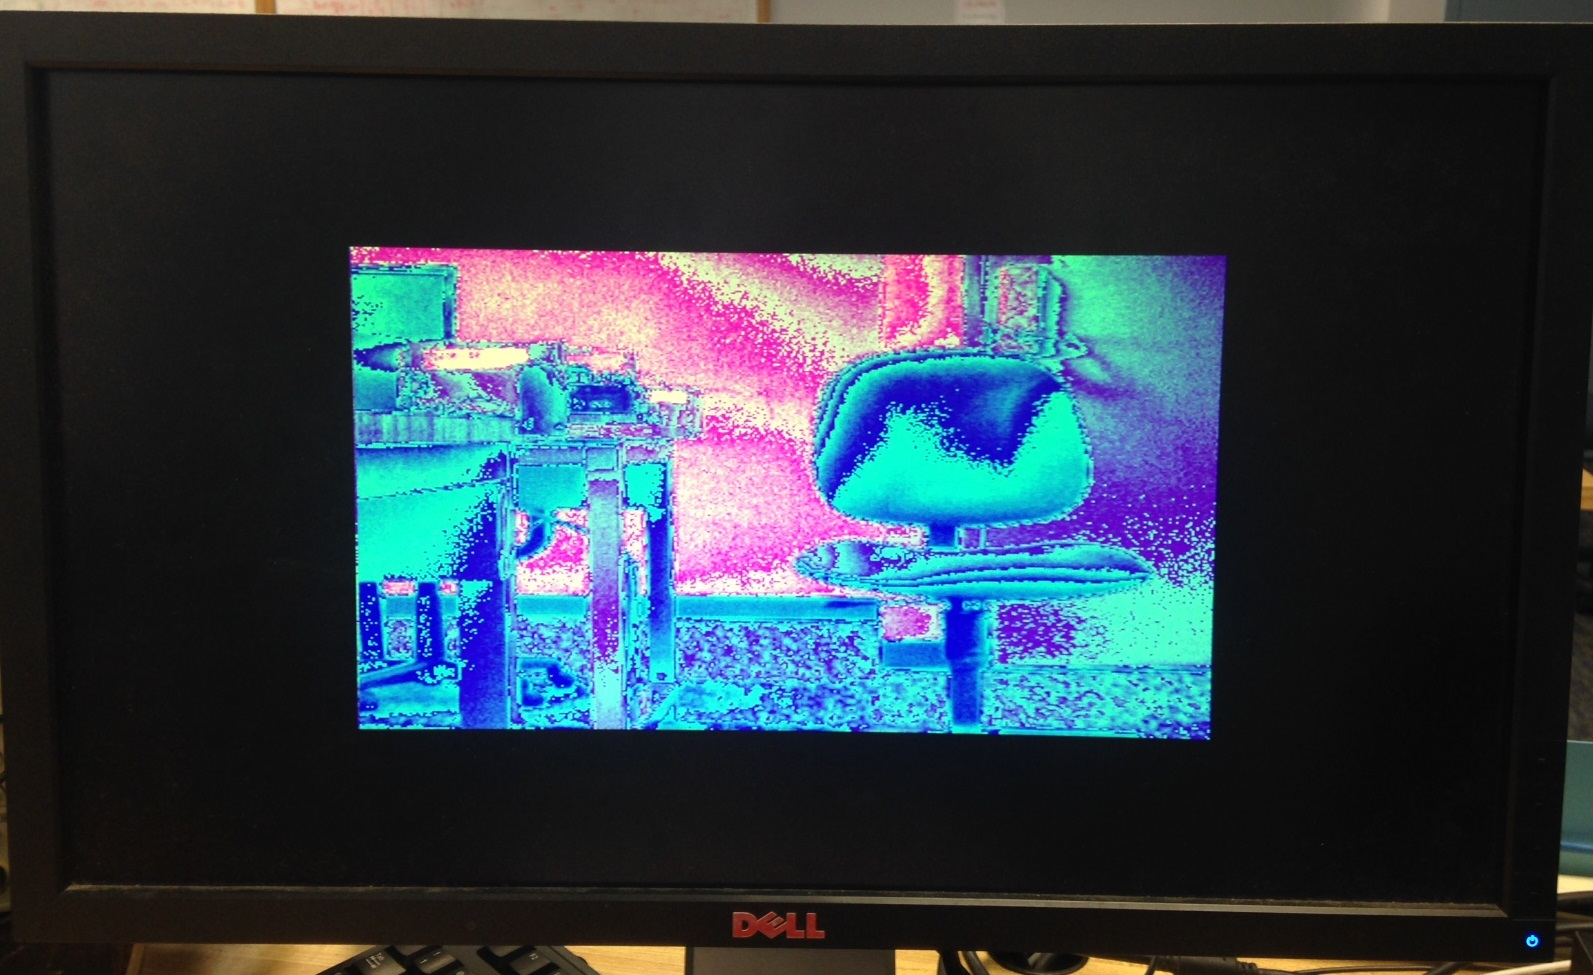
\includegraphics[width=1\linewidth]{camera_mode.JPG}
	}
	\caption{Raw Camera Data Mode}
	\label{camOutMode}
\end{figure}
\par
The output of the hardware disparity implementation was verified by using a VGA display driver to show the algorithm's output in real time, as demonstrated in Figure \ref{disparityFin}. With this output mode successfully implemented, the disparity and camera controller modules were then added into a finalized design that incorporated the IMU and Rangefinder modules. Each of these modules may be found in Appendix items \ref{finalCamBuf} and \ref{finalDisparity}, respectively. 
\par
\begin{figure}[H] 
	\begin{subfigure}{0.5\textwidth}
	\centering
		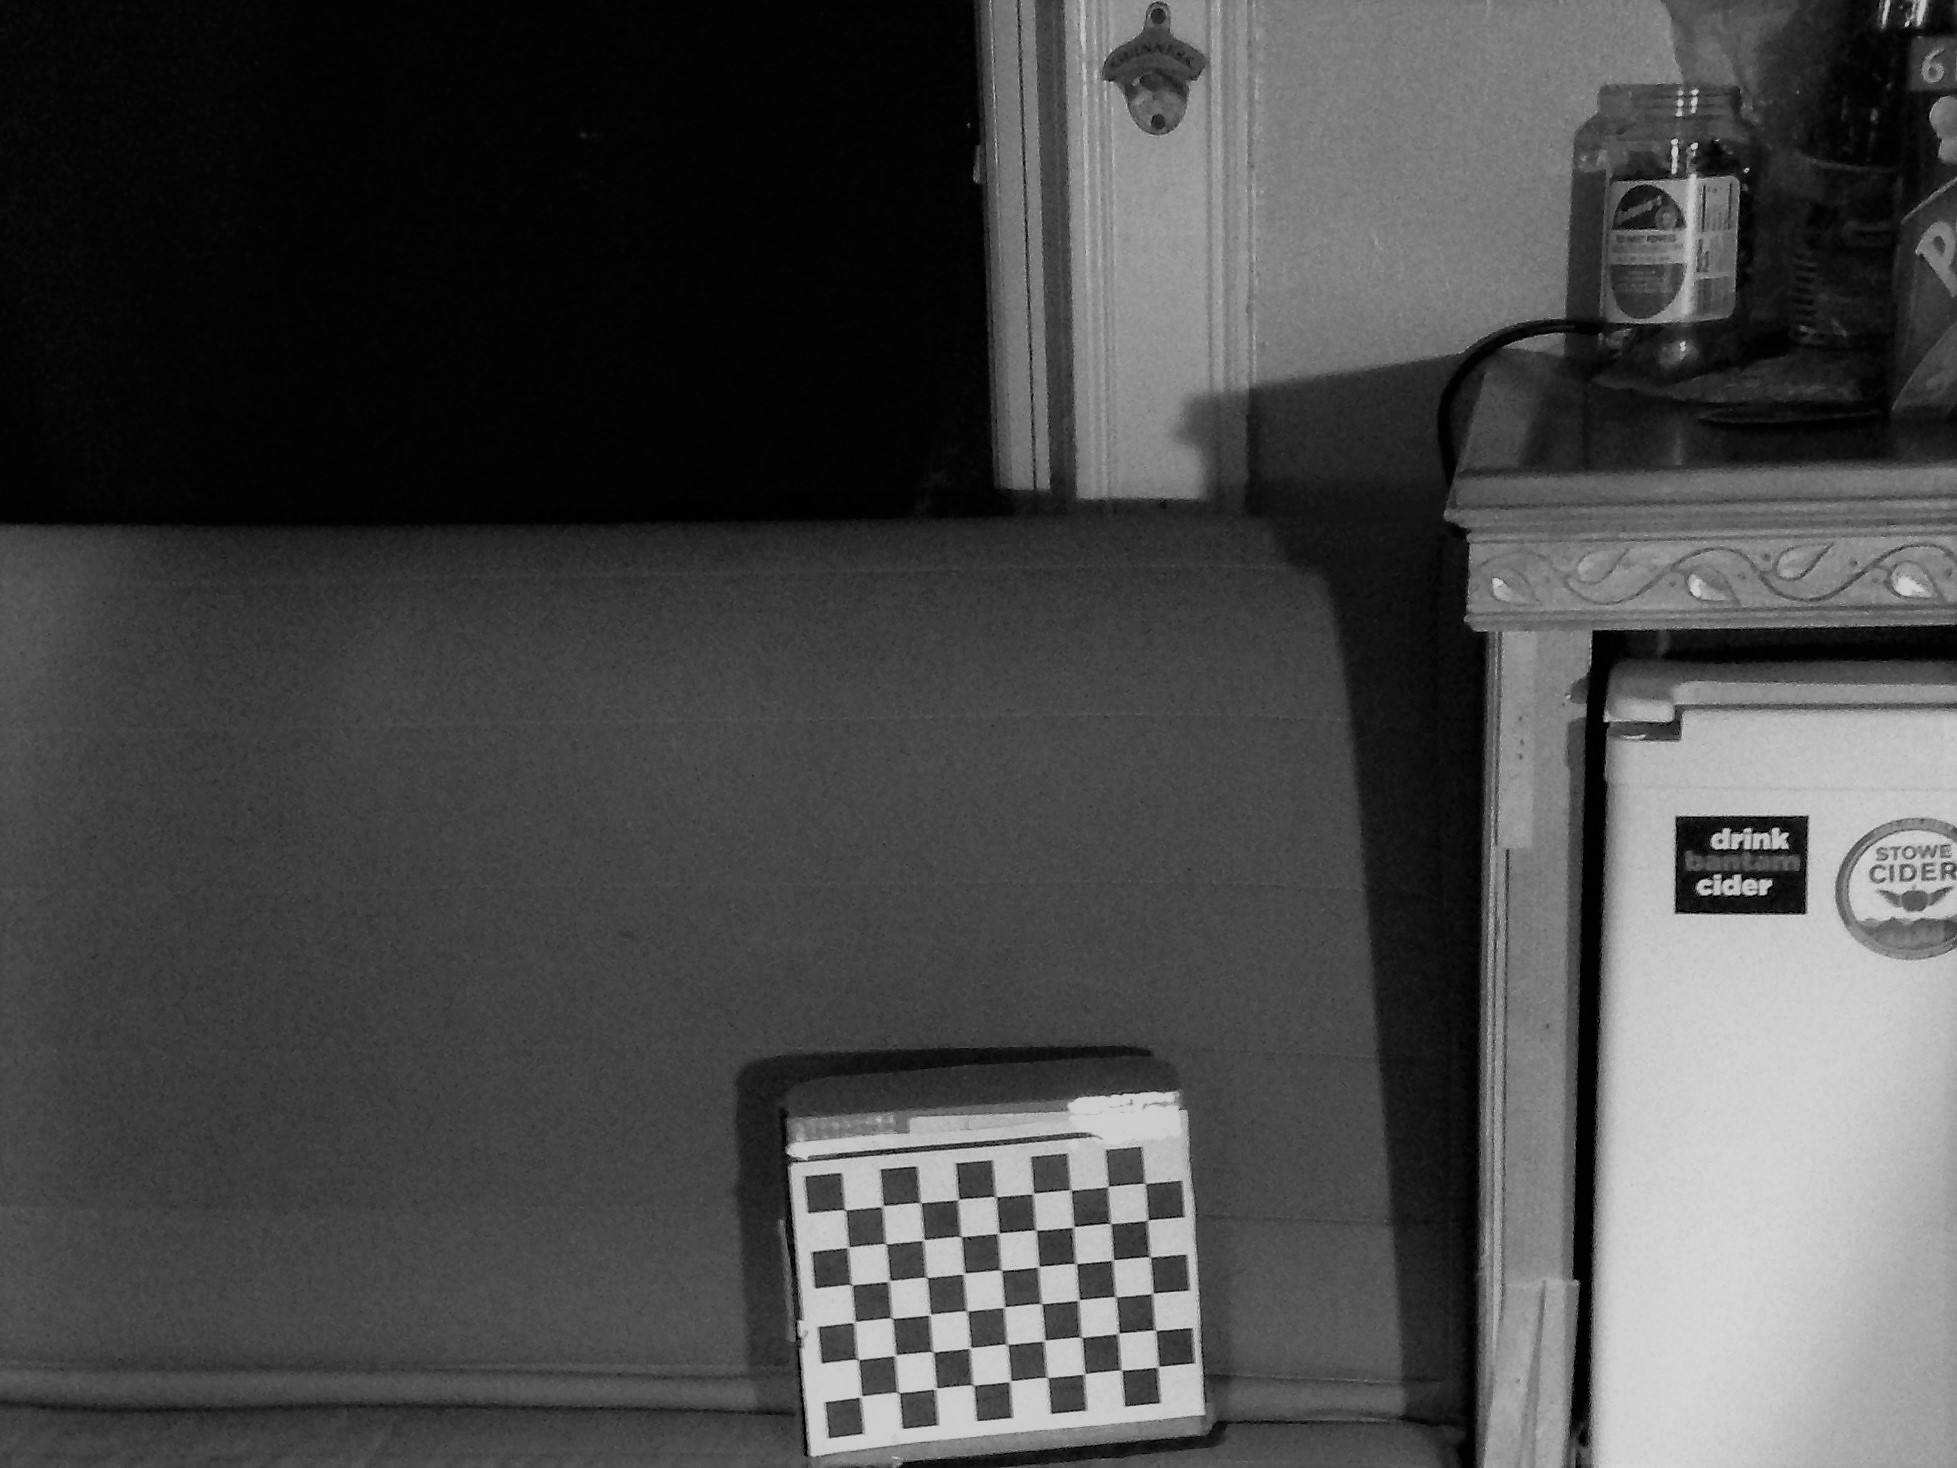
\includegraphics[width=0.8\linewidth]{disparity_rtView.JPG}
		\caption{Device View}
	\end{subfigure}
	\begin{subfigure}{0.5\textwidth}
	\centering
		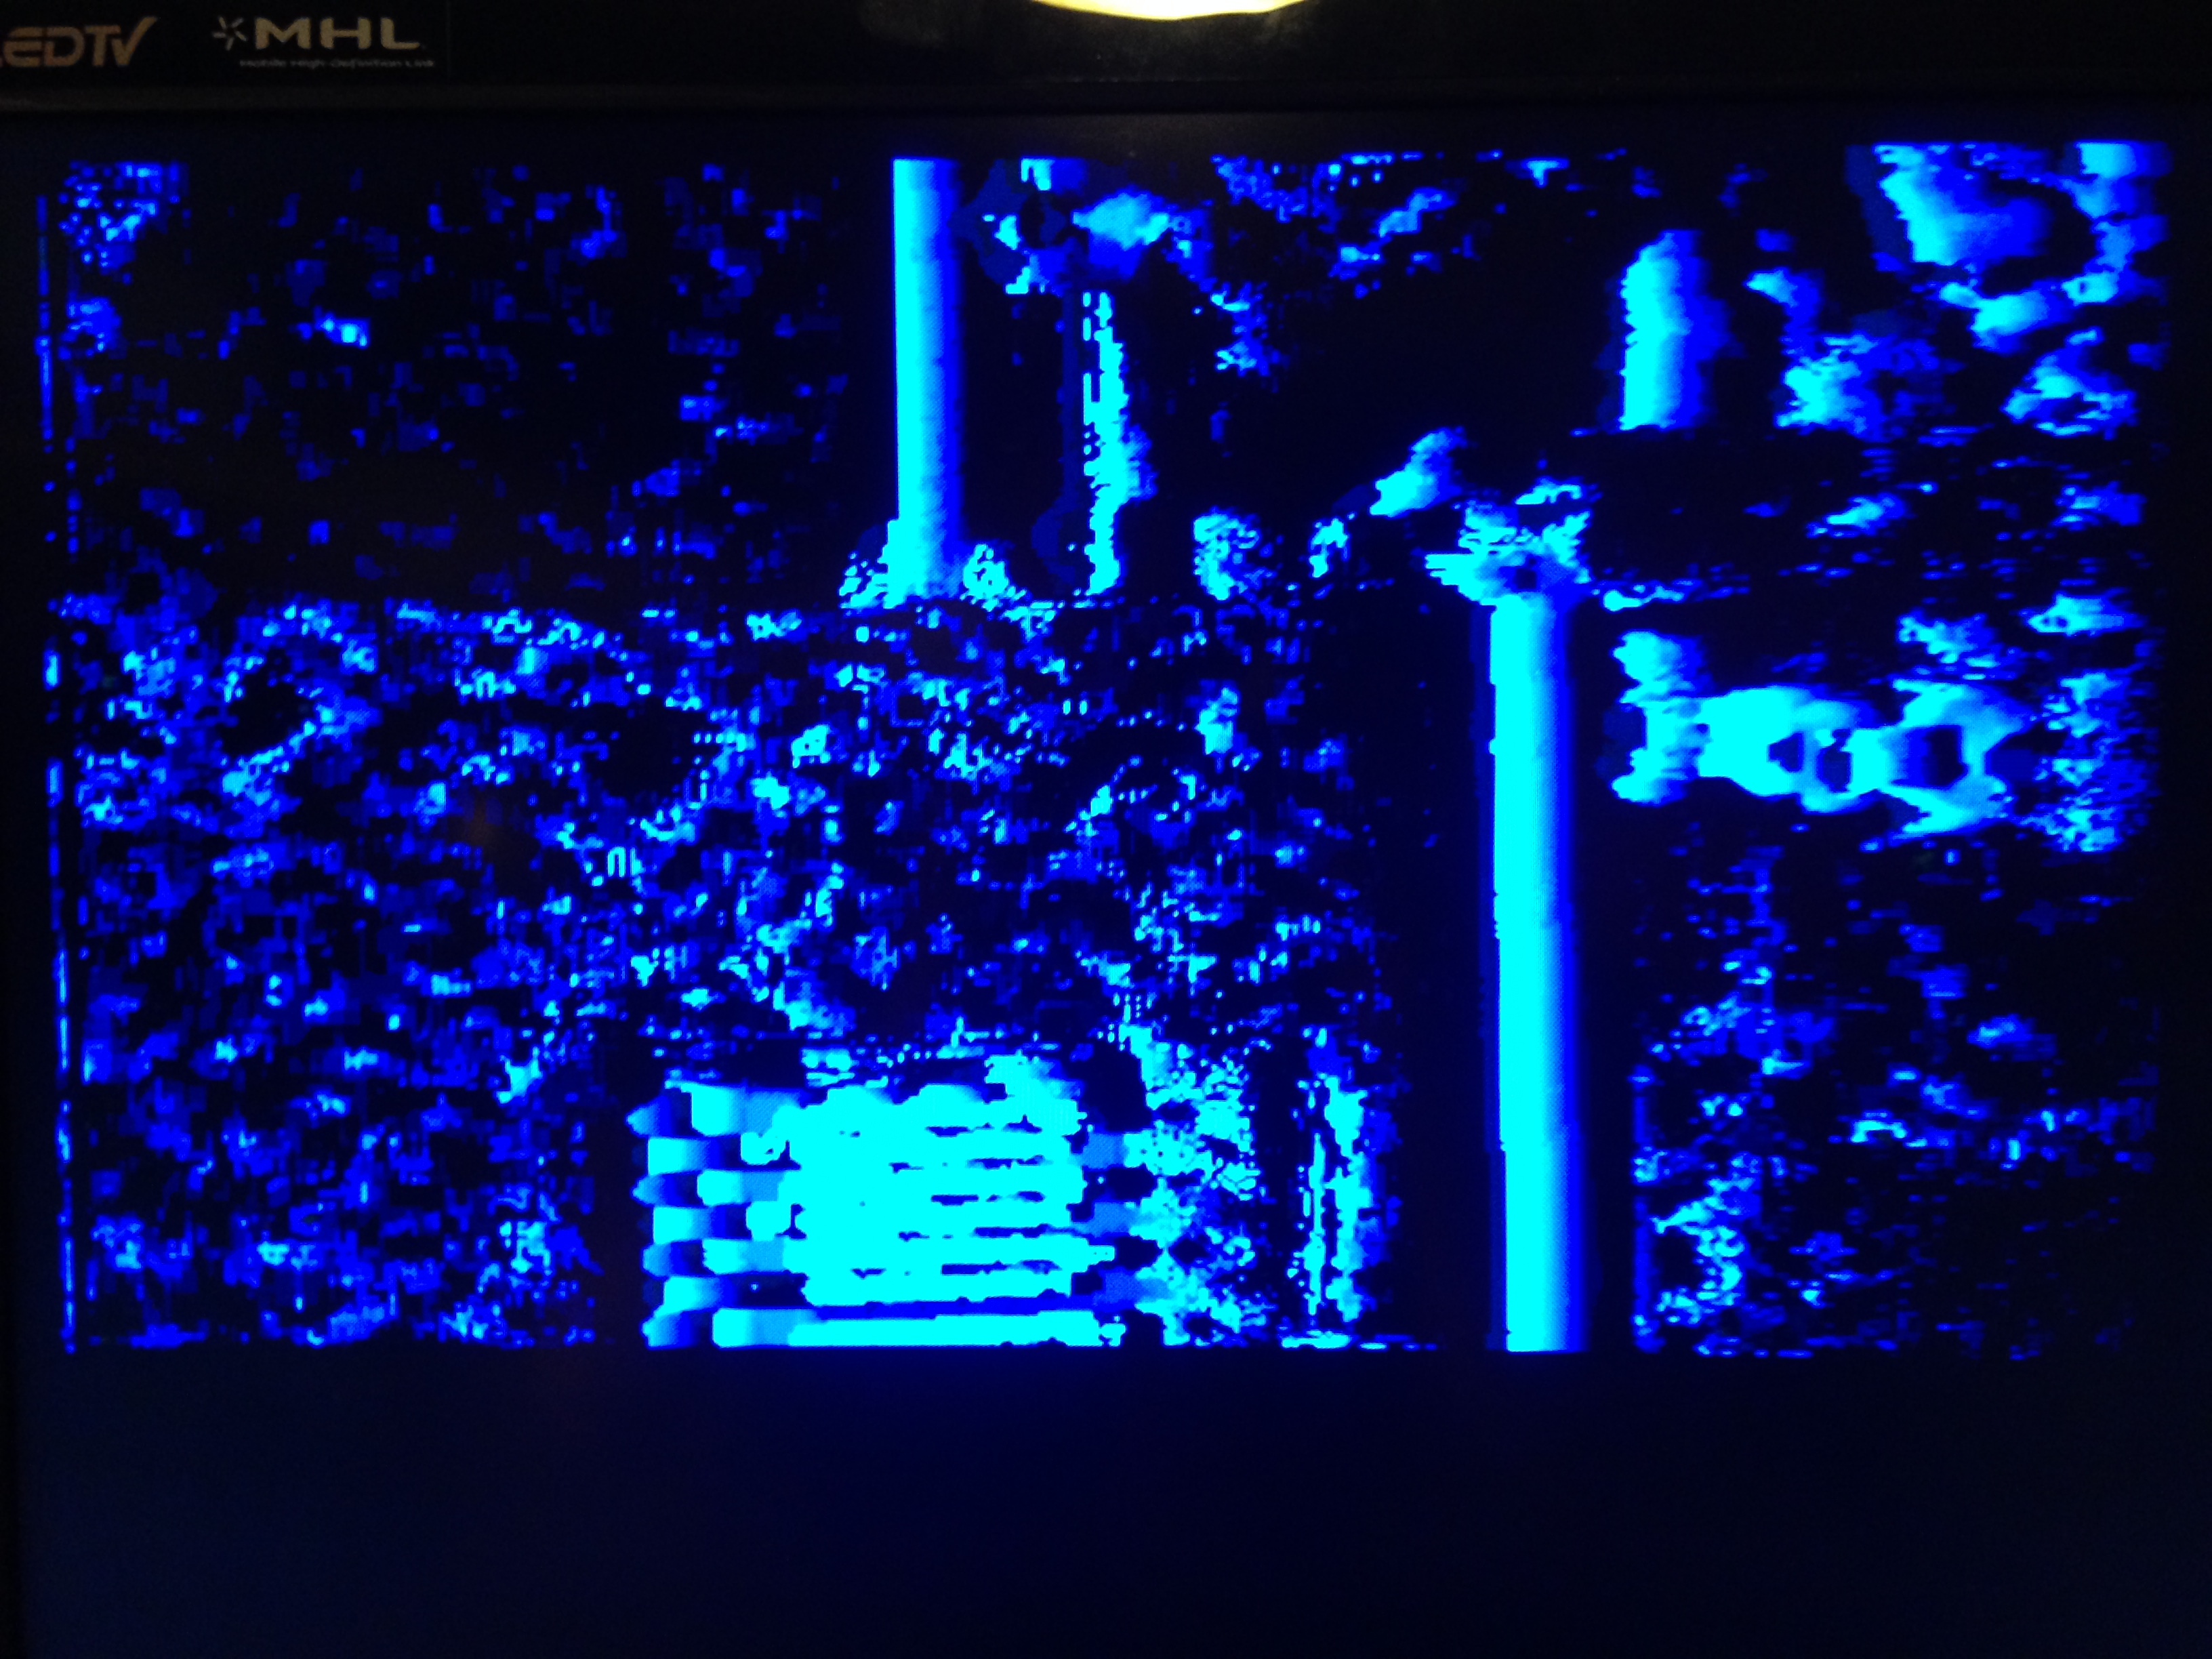
\includegraphics[width=0.8\linewidth]{disparity_rt.JPG}
		\caption{Resultant Disparity}
	\end{subfigure}
	\caption{Disparity Algorithm Output}
	\label{disparityFin}
\end{figure}